
% *** Authors should verify (and, if needed, correct) their LaTeX system  ***
% *** with the testflow diagnostic prior to trusting their LaTeX platform ***
% *** with production work. IEEE's font choices can trigger bugs that do  ***
% *** not appear when using other class files.                            ***
% The testflow support page is at:
% http://www.michaelshell.org/tex/testflow/

\documentclass[conference, compsoc]{IEEEtran}

\usepackage{graphicx}
\usepackage{color}
\usepackage{bussproofs} 
\usepackage{listings}
%\message{<Paul Taylor's Proof Trees, 2 August 1996>}
%% Build proof tree for Natural Deduction, Sequent Calculus, etc.
%% WITH SHORTENING OF PROOF RULES!
%% Paul Taylor, begun 10 Oct 1989
%% *** THIS IS ONLY A PRELIMINARY VERSION AND THINGS MAY CHANGE! ***
%%
%% 2 Aug 1996: fixed \mscount and \proofdotnumber
%%
%%      \prooftree
%%              hyp1            produces:
%%              hyp2
%%              hyp3            hyp1    hyp2    hyp3
%%      \justifies              -------------------- rulename
%%              concl                   concl
%%      \thickness=0.08em
%%      \shiftright 2em
%%      \using
%%              rulename
%%      \endprooftree
%%
%% where the hypotheses may be similar structures or just formulae.
%%
%% To get a vertical string of dots instead of the proof rule, do
%%
%%      \prooftree                      which produces:
%%              [hyp]
%%      \using                                  [hyp]
%%              name                              .
%%      \proofdotseparation=1.2ex                 .name
%%      \proofdotnumber=4                         .
%%      \leadsto                                  .
%%              concl                           concl
%%      \endprooftree
%%
%% Within a prooftree, \[ and \] may be used instead of \prooftree and
%% \endprooftree; this is not permitted at the outer level because it
%% conflicts with LaTeX. Also,
%%      \Justifies
%% produces a double line. In LaTeX you can use \begin{prooftree} and
%% \end{prootree} at the outer level (however this will not work for the inner
%% levels, but in any case why would you want to be so verbose?).
%%
%% All of of the keywords except \prooftree and \endprooftree are optional
%% and may appear in any order. They may also be combined in \newcommand's
%% eg "\def\Cut{\using\sf cut\thickness.08em\justifies}" with the abbreviation
%% "\prooftree hyp1 hyp2 \Cut \concl \endprooftree". This is recommended and
%% some standard abbreviations will be found at the end of this file.
%%
%% \thickness specifies the breadth of the rule in any units, although
%% font-relative units such as "ex" or "em" are preferable.
%% It may optionally be followed by "=".
%% \proofrulebreadth=.08em or \setlength\proofrulebreadth{.08em} may also be
%% used either in place of \thickness or globally; the default is 0.04em.
%% \proofdotseparation and \proofdotnumber control the size of the
%% string of dots
%%
%% If proof trees and formulae are mixed, some explicit spacing is needed,
%% but don't put anything to the left of the left-most (or the right of
%% the right-most) hypothesis, or put it in braces, because this will cause
%% the indentation to be lost.
%%
%% By default the conclusion is centered wrt the left-most and right-most
%% immediate hypotheses (not their proofs); \shiftright or \shiftleft moves
%% it relative to this position. (Not sure about this specification or how
%% it should affect spreading of proof tree.)
%
% global assignments to dimensions seem to have the effect of stretching
% diagrams horizontally.
%
%%==========================================================================

\def\introrule{{\cal I}}\def\elimrule{{\cal E}}%%
\def\andintro{\using{\land}\introrule\justifies}%%
\def\impelim{\using{\Rightarrow}\elimrule\justifies}%%
\def\allintro{\using{\forall}\introrule\justifies}%%
\def\allelim{\using{\forall}\elimrule\justifies}%%
\def\falseelim{\using{\bot}\elimrule\justifies}%%
\def\existsintro{\using{\exists}\introrule\justifies}%%

%% #1 is meant to be 1 or 2 for the first or second formula
\def\andelim#1{\using{\land}#1\elimrule\justifies}%%
\def\orintro#1{\using{\lor}#1\introrule\justifies}%%

%% #1 is meant to be a label corresponding to the discharged hypothesis/es
\def\impintro#1{\using{\Rightarrow}\introrule_{#1}\justifies}%%
\def\orelim#1{\using{\lor}\elimrule_{#1}\justifies}%%
\def\existselim#1{\using{\exists}\elimrule_{#1}\justifies}

%%==========================================================================

\newdimen\proofrulebreadth \proofrulebreadth=.05em
\newdimen\proofdotseparation \proofdotseparation=1.25ex
\newdimen\proofrulebaseline \proofrulebaseline=2ex
\newcount\proofdotnumber \proofdotnumber=3
\let\then\relax
\def\hfi{\hskip0pt plus.0001fil}
\mathchardef\squigto="3A3B
%
% flag where we are
\newif\ifinsideprooftree\insideprooftreefalse
\newif\ifonleftofproofrule\onleftofproofrulefalse
\newif\ifproofdots\proofdotsfalse
\newif\ifdoubleproof\doubleprooffalse
\let\wereinproofbit\relax
%
% dimensions and boxes of bits
\newdimen\shortenproofleft
\newdimen\shortenproofright
\newdimen\proofbelowshift
\newbox\proofabove
\newbox\proofbelow
\newbox\proofrulename
%
% miscellaneous commands for setting values
\def\shiftproofbelow{\let\next\relax\afterassignment\setshiftproofbelow\dimen0 }
\def\shiftproofbelowneg{\def\next{\multiply\dimen0 by-1 }%
\afterassignment\setshiftproofbelow\dimen0 }
\def\setshiftproofbelow{\next\proofbelowshift=\dimen0 }
\def\setproofrulebreadth{\proofrulebreadth}

%=============================================================================
\def\prooftree{% NESTED ZERO (\ifonleftofproofrule)
%
% first find out whether we're at the left-hand end of a proof rule
\ifnum  \lastpenalty=1
\then   \unpenalty
\else   \onleftofproofrulefalse
\fi
%
% some space on left (except if we're on left, and no infinity for outermost)
\ifonleftofproofrule
\else   \ifinsideprooftree
        \then   \hskip.5em plus1fil
        \fi
\fi
%
% begin our proof tree environment
\bgroup% NESTED ONE (\proofbelow, \proofrulename, \proofabove,
%               \shortenproofleft, \shortenproofright, \proofrulebreadth)
\setbox\proofbelow=\hbox{}\setbox\proofrulename=\hbox{}%
\let\justifies\proofover\let\leadsto\proofoverdots\let\Justifies\proofoverdbl
\let\using\proofusing\let\[\prooftree
\ifinsideprooftree\let\]\endprooftree\fi
\proofdotsfalse\doubleprooffalse
\let\thickness\setproofrulebreadth
\let\shiftright\shiftproofbelow \let\shift\shiftproofbelow
\let\shiftleft\shiftproofbelowneg
\let\ifwasinsideprooftree\ifinsideprooftree
\insideprooftreetrue
%
% now begin to set the top of the rule (definitions local to it)
\setbox\proofabove=\hbox\bgroup$\displaystyle % NESTED TWO
\let\wereinproofbit\prooftree
%
% these local variables will be copied out:
\shortenproofleft=0pt \shortenproofright=0pt \proofbelowshift=0pt
%
% flags to enable inner proof tree to detect if on left:
\onleftofproofruletrue\penalty1
}

%=============================================================================
% end whatever box and copy crucial values out of it
\def\eproofbit{% NESTED TWO
%
% various hacks applicable to hypothesis list 
\ifx    \wereinproofbit\prooftree
\then   \ifcase \lastpenalty
        \then   \shortenproofright=0pt  % 0: some other object, no indentation
        \or     \unpenalty\hfil         % 1: empty hypotheses, just glue
        \or     \unpenalty\unskip       % 2: just had a tree, remove glue
        \else   \shortenproofright=0pt  % eh?
        \fi
\fi
%
% pass out crucial values from scope
\global\dimen0=\shortenproofleft
\global\dimen1=\shortenproofright
\global\dimen2=\proofrulebreadth
\global\dimen3=\proofbelowshift
\global\dimen4=\proofdotseparation
\global\count255=\proofdotnumber
%
% end the box
$\egroup  % NESTED ONE
%
% restore the values
\shortenproofleft=\dimen0
\shortenproofright=\dimen1
\proofrulebreadth=\dimen2
\proofbelowshift=\dimen3
\proofdotseparation=\dimen4
\proofdotnumber=\count255
}

%=============================================================================
\def\proofover{% NESTED TWO
\eproofbit % NESTED ONE
\setbox\proofbelow=\hbox\bgroup % NESTED TWO
\let\wereinproofbit\proofover
$\displaystyle
}%
%
%=============================================================================
\def\proofoverdbl{% NESTED TWO
\eproofbit % NESTED ONE
\doubleprooftrue
\setbox\proofbelow=\hbox\bgroup % NESTED TWO
\let\wereinproofbit\proofoverdbl
$\displaystyle
}%
%
%=============================================================================
\def\proofoverdots{% NESTED TWO
\eproofbit % NESTED ONE
\proofdotstrue
\setbox\proofbelow=\hbox\bgroup % NESTED TWO
\let\wereinproofbit\proofoverdots
$\displaystyle
}%
%
%=============================================================================
\def\proofusing{% NESTED TWO
\eproofbit % NESTED ONE
\setbox\proofrulename=\hbox\bgroup % NESTED TWO
\let\wereinproofbit\proofusing
\kern0.3em$
}

%=============================================================================
\def\endprooftree{% NESTED TWO
\eproofbit % NESTED ONE
% \dimen0 =     length of proof rule
% \dimen1 =     indentation of conclusion wrt rule
% \dimen2 =     new \shortenproofleft, ie indentation of conclusion
% \dimen3 =     new \shortenproofright, ie
%                space on right of conclusion to end of tree
% \dimen4 =     space on right of conclusion below rule
  \dimen5 =0pt% spread of hypotheses
% \dimen6, \dimen7 = height & depth of rule
%
% length of rule needed by proof above
\dimen0=\wd\proofabove \advance\dimen0-\shortenproofleft
\advance\dimen0-\shortenproofright
%
% amount of spare space below
\dimen1=.5\dimen0 \advance\dimen1-.5\wd\proofbelow
\dimen4=\dimen1
\advance\dimen1\proofbelowshift \advance\dimen4-\proofbelowshift
%
% conclusion sticks out to left of immediate hypotheses
\ifdim  \dimen1<0pt
\then   \advance\shortenproofleft\dimen1
        \advance\dimen0-\dimen1
        \dimen1=0pt
%       now it sticks out to left of tree!
        \ifdim  \shortenproofleft<0pt
        \then   \setbox\proofabove=\hbox{%
                        \kern-\shortenproofleft\unhbox\proofabove}%
                \shortenproofleft=0pt
        \fi
\fi
%
% and to the right
\ifdim  \dimen4<0pt
\then   \advance\shortenproofright\dimen4
        \advance\dimen0-\dimen4
        \dimen4=0pt
\fi
%
% make sure enough space for label
\ifdim  \shortenproofright<\wd\proofrulename
\then   \shortenproofright=\wd\proofrulename
\fi
%
% calculate new indentations
\dimen2=\shortenproofleft \advance\dimen2 by\dimen1
\dimen3=\shortenproofright\advance\dimen3 by\dimen4
%
% make the rule or dots, with name attached
\ifproofdots
\then
        \dimen6=\shortenproofleft \advance\dimen6 .5\dimen0
        \setbox1=\vbox to\proofdotseparation{\vss\hbox{$\cdot$}\vss}%
        \setbox0=\hbox{%
                \advance\dimen6-.5\wd1
                \kern\dimen6
                $\vcenter to\proofdotnumber\proofdotseparation
                        {\leaders\box1\vfill}$%
                \unhbox\proofrulename}%
\else   \dimen6=\fontdimen22\the\textfont2 % height of maths axis
        \dimen7=\dimen6
        \advance\dimen6by.5\proofrulebreadth
        \advance\dimen7by-.5\proofrulebreadth
        \setbox0=\hbox{%
                \kern\shortenproofleft
                \ifdoubleproof
                \then   \hbox to\dimen0{%
                        $\mathsurround0pt\mathord=\mkern-6mu%
                        \cleaders\hbox{$\mkern-2mu=\mkern-2mu$}\hfill
                        \mkern-6mu\mathord=$}%
                \else   \vrule height\dimen6 depth-\dimen7 width\dimen0
                \fi
                \unhbox\proofrulename}%
        \ht0=\dimen6 \dp0=-\dimen7
\fi
%
% set up to centre outermost tree only
\let\doll\relax
\ifwasinsideprooftree
\then   \let\VBOX\vbox
\else   \ifmmode\else$\let\doll=$\fi
        \let\VBOX\vcenter
\fi
% this \vbox or \vcenter is the actual output:
\VBOX   {\baselineskip\proofrulebaseline \lineskip.2ex
        \expandafter\lineskiplimit\ifproofdots0ex\else-0.6ex\fi
        \hbox   spread\dimen5   {\hfi\unhbox\proofabove\hfi}%
        \hbox{\box0}%
        \hbox   {\kern\dimen2 \box\proofbelow}}\doll%
%
% pass new indentations out of scope
\global\dimen2=\dimen2
\global\dimen3=\dimen3
\egroup % NESTED ZERO
\ifonleftofproofrule
\then   \shortenproofleft=\dimen2
\fi
\shortenproofright=\dimen3
%
% some space on right and flag we've just made a tree
\onleftofproofrulefalse
\ifinsideprooftree
\then   \hskip.5em plus 1fil \penalty2
\fi
}

%==========================================================================
% IDEAS
% 1.    Specification of \shiftright and how to spread trees.
% 2.    Spacing command \m which causes 1em+1fil spacing, over-riding
%       exisiting space on sides of trees and not affecting the
%       detection of being on the left or right.
% 3.    Hack using \@currenvir to detect LaTeX environment; have to
%       use \aftergroup to pass \shortenproofleft/right out.
% 4.    (Pie in the sky) detect how much trees can be "tucked in"
% 5.    Discharged hypotheses (diagonal lines).


\usepackage{listings}
\usepackage{keyval}
\usepackage{ifthen}
\usepackage{alltt}

% alguns comandos
\newcommand{\Fix}[1]{\textbf{[[#1]]}}   
\newcommand{\truee}{\mathbf{true}}
\newtheorem{refine}{\bf{Refactoring}}
\newenvironment{refinement}[1]
   {\begin{refine} \normalfont \lawName{#1} \\ \noindent}
   {\end{refine}}
\newcommand{\bfoo}{\bfooc{true}}
\newcommand{\efoo}{\efooc{true}}
\newcommand{\bfooc}[1]
   {\ifthenelse{\equal{#1}{true}}{\begin{alltt}}{\begin{forget}}}
\newcommand{\efooc}[1]
    {\ifthenelse{\equal{#1}{true}}{\end{alltt}}{\end{forget}}}

\newcommand{\cc}[1]{\ensuremath{#1}}


       
\begin{document}

\lstset{language=Haskell, basicstyle=\small,aboveskip=10pt}


%
% paper title
% can use linebreaks \\ within to get better formatting as desired
\title{Detecting Errors and Bad Smells in Feature Modeling}


% author names and affiliations
% use a multiple column layout for up to two different
% affiliations

\author{\IEEEauthorblockN{Rodrigo Bonif\'{a}cio, Leopoldo Teixeira, Paulo Borba}
\IEEEauthorblockA{Informatics Center\\
Federal University of Pernambuco\\
Recife, Brazil\\
\{rba2,lmt,phmb\}@cin.ufpe.br}
\and
\IEEEauthorblockN{Rohit Gheyi, Tiago Massoni }
\IEEEauthorblockA{Department of Computer Science\\
Federal University of Campina Grande\\
Campina Grande, Brazil\\
\{rohit, massoni\}@dsc.ufcg.edu.br}
}

% conference papers do not typically use \thanks and this command
% is locked out in conference mode. If really needed, such as for
% the acknowledgment of grants, issue a \IEEEoverridecommandlockouts
% after \documentclass

% for over three affiliations, or if they all won't fit within the width
% of the page, use this alternative format:
% 
%\author{\IEEEauthorblockN{Michael Shell\IEEEauthorrefmark{1},
%Homer Simpson\IEEEauthorrefmark{2},
%James Kirk\IEEEauthorrefmark{3}, 
%Montgomery Scott\IEEEauthorrefmark{3} and
%Eldon Tyrell\IEEEauthorrefmark{4}}
%\IEEEauthorblockA{\IEEEauthorrefmark{1}School of Electrical and Computer Engineering\\
%Georgia Institute of Technology,
%Atlanta, Georgia 30332--0250\\ Email: see http://www.michaelshell.org/contact.html}
%\IEEEauthorblockA{\IEEEauthorrefmark{2}Twentieth Century Fox, Springfield, USA\\
%Email: homer@thesimpsons.com}
%\IEEEauthorblockA{\IEEEauthorrefmark{3}Starfleet Academy, San Francisco, California 96678-2391\\
%Telephone: (800) 555--1212, Fax: (888) 555--1212}
%\IEEEauthorblockA{\IEEEauthorrefmark{4}Tyrell Inc., 123 Replicant Street, Los Angeles, California 90210--4321}}


% make the title area
\maketitle


\begin{abstract}
% contexto
Feature modeling is a worth and widespread approach for 
representing the common and variant capabilities of a software 
product line. 
% problema
However, besides the recent proposals for feature model semantics, 
there is a lack of definition regarding the characteristics of a 
well typed feature model. Moreover, even being well typed, models
may be badly structured. There are no catalog of bad smells for feature models
in order to help domain analysts. 
% solu��o
In this paper, we go a step further in this direction, formalizing 
typing rules and bad smells for feature modeling and presenting 
an automated approach for revealing these problems. Moreover, we propose
FM refactorings for removing the bad smells.
% avalia��o
%Our proposal 
%approach efficiently reveals type errors and bad-smells in models with 
% acho que no m�nimo temos que avaliar em 5000 diante dos papers atuais
%at most 5000 features. 
% aplica��o
This formalization can be useful for showing that FM transformations, such as
refactorings, do not introduce type errors.
% colocar mais aplica��es
\end{abstract}

\section{Introduction}
The support for variation points enables product customization from a set of
reusable assets~\cite{Pohl:2005aa}. However, variability management, due to its
inherent crosscutting nature, is a common challenge in software product line
(SPL) adoption~\cite{Clements:2001aa,Pohl:2005aa}. First, nontrivial features
often require associated variation points to be scattered through SPL artifacts.
Second, some approaches include product variant and configuration information
inside artifacts. Both problems can be observed for use case scenario
specifications.

Several authors have proposed the use of \emph{aspect-oriented} mechanisms to
better modularize the specification of crosscutting
concerns~\cite{Moreira:2004aa,Chitchyan:2007aa}. These techniques minimizes the
first problem, since they can be used to modularize the specification of certain
features. However, they do not support the different sources of variability that
occur in SPL requirements. With respect to the second problem, existing
approaches~\cite{Bertolino:2003aa,Eriksson:2005aa} proposed to
scenario variability management do not offer a clear separation between
variability management and scenario specification. As a consequence, in the case
where details about product variants are tangled with use case scenarios, the
removal of one variant from the product line requires changes to all related
scenarios. In summary, it is difficult to evolve both representations.

So in this paper we go beyond the common-variant scenario composition issues and
consider a more encompassing notion of variability management, including
artifacts such as feature models~\cite{Gheyi:2006aa,Czarnecki:2000aa} and
configuration knowledge~\cite{Czarnecki:2000aa,Pohl:2005aa}. We explain this as a
crosscutting phenomenon, using Masuhara and Kiczales work~\cite{Masuhara:2003aa},
and apply this view of \emph{variability management as crosscutting} for
modularizing SPL use case scenarios, providing the necessary separation between
variability and scenario specification concerns. We also formalize the derivation
of product specific scenarios in our approach, as demanded by current SPL
generative practices~\cite{Krueger:2006aa}. This formalization is based on our
framework for modeling the composition process of scenario variabilities with
feature models, product configuration, and configuration knowledge. Besides
supporting the mentioned separation of concerns, this framework helps to
precisely specify how to weave the different representations in order to generate
specific scenarios for a SPL member. Therefore, the main contributions of this
work are the following:

\begin{itemize}
\item Characterization of the languages of variability management as a
crosscutting concern and, in this way, proposing an approach where variability
concerns are separated from other concerns (Section~\ref{sec:svmc}).

%Although this work focus on requirement artifacts, more specifically use case scenarios, we argue that such separation is also valid for other SPL artifacts. Actually, it has already been claimed for source code~\cite{Alves:2006aa,Apel:2006aa}, without considering the importance of variability artifacts.

\item A framework for modeling the composition process of scenario variability
mechanisms (Section~\ref{sec:modeling-framework}). Differently from existing
works~\cite{Morin:2008aa,Groher:2008aa}, this framework gives a basis for
describing variability as crosscutting mechanisms, at the same time it considers the contribution of different input
languages: feature models, product configuration, configuration knowledge and SPL use case
model. Moreover, the reference implementation provided for each variability
mechanism corresponds to the essencial parts of a tool environment for scenario
variability management. In this paper we focus just in these essencials.

\item Specification of three {\color{red}sources of variability for use case
scenarios: variability in function (Section~\ref{sub:pd-weaver}),
variability in data (Section~\ref{sub:bind-weaver}), and variability in control
flow (Section~\ref{sub:sc-weaver})}. This specification provides a more formal
semantic representation when compared to existing works; which is an important property
for supporting the automatic derivation of product specific artifacts.
\end{itemize}

{\color{red}The sources of
variability (or kinds of composition) for use case scenarios presented here are
not complete. However, our modeling framework is able to represent
other interesting sources of variability, such as context-aware adaptability.
Additionally, since the word \emph{scenario} has different meanings in software
engineering, we want to make clear that in the remainder of this paper the term
\emph{scenario} corresponds to textual use case scenarios. We explain the structure
used for specifying scenarios in Section~\ref{sub:spl-uc}}.

Since our concept of crosscutting mechanism is based on Masuhara and Kiczales
work~\cite{Masuhara:2003aa}, a smaller contribution of this paper is to apply
their ideas to the languages of variability management,  reinforcing the
generality of their model, which was originally instantiated only for mechanisms
of aspect-oriented programming languages. Based on their view of crosscutting, we
can reason about variability management as a crosscutting concern that involves
different input specifications that contribute to derive a specific member of a
given SPL. 

Finally, we evaluate our approach (Section~\ref{sec:evaluation}) by comparing it
to alternative approaches using different product lines. We also relate our work
with other research topics (Section~\ref{sec:related}) and present our concluding
remarks (Section~\ref{sec:conclusions}). 
\section{Type System}
\label{sec:type-checker}

One of the main concerns in our research work is \emph{type safety} in feature models, in order to prevent erroneous or undesirable analysis results. We consider a feature model well-typed if a number of well-formation constraints are obeyed. We present these rules in this section, both informally and using a formalization language with conventional notation mixed with the PVS language~\cite{Owre:2009aa}. Notice that this is a minimal set of constraints, as derived from our knowledge about the requirements for verifying that a selection of features is a valid member of a feature model.

We begin by providing a formal definition for feature models, which are composed of a root feature, relations, features and formulae. While \texttt{Feature} is an uninterpreted type -- with a name -- relation is a PVS datatype with four distinct classes: optional (\texttt{OPT\_REL}), mandatory (\texttt{MAND\_REL}), alternative (\texttt{ALT\_REL}) and Or-feature (\texttt{OR\_REL}). While the first two types are defined between two features, the latter are defined between a parent and a set of child features. Furthermore, we consider a set of formulae for defining constraints over the feature model (in this case, core formulae only, such as negation, conjunction and implication).

\bfoo{\small
  FM: type = [# 
    root: Feature,
    relations: set[Relation]
    features: set[Feature], 
    formulae: set[Formula] 
  #]

  Relation: datatype
  begin 
  	OPT_REL(p,c: Feature):OPT?:Relation
  	MAND_REL(p,c: Feature):MAND?:Relation
  	ALT_REL(p: Feature,c:set[Feature]):
  	  ALT?:Relation
  	OR_REL(p: Feature,c:set[Feature]):
  	  OR?:Relation
	end Relation
	
	Formula : datatype
    TRUE_FORMULA:TRUE?:Formula
    FALSE_FORMULA:FALSE?:Formula
    NAME_FORMULA(n: Name):NAME?:Formula
    NOT_FORMULA(f: Formula):NOT?:Formula
    AND_FORMULA(f0,f1: Formula):
        AND?:Formula
    IMPLIES_FORMULA(f0,f1:Formula):
        IMPLIES?:Formula
  end Formula
}\efoo%

A feature model is well typed iff its feature tree is well formed and its constraints are well typed. A feature tree must satisfy the following well-formedness rules:
\begin{itemize}
	\item there must exist exactly one root feature (already contemplated in the previous \texttt{FM} definition);
	\item features must form a tree, as a connected and acyclic graph;
	\item feature names must be unique;
	\item all relations are well formed.
\end{itemize}
%{\bf (F.)} Consider $f \in F$, where F is the set of features defined in a feature tree. If $f$ is a \emph{Basic-feature}, it will always be well typed. Otherwise, if $f$ is an \emph{Or-feature} or an \emph{Alternative-feature}, $f$ will be well typed iff $children (f) \neq \emptyset$. 

\bfoo{\small
  wellTyped(fm: FM): boolean =
    wellFormednessRules(fm) \cc{\wedge} 
    wellTypedFormulae(fm)

  wellFormednessRules(fm: FM): bool = 
    tree(fm) \cc{\wedge} uniqueFeatureNames(fm) \cc{\wedge}
    wellFormedRelations(fm)

}\efoo

For the \texttt{tree} predicate, two other auxiliary predicates must be valid: all features must constitute a graph that is both \emph{acyclic} and \emph{connected}; these predicates use the \texttt{children} function, which returns the transitive closure of the set of relations within the feature model. In addition, relations are well-formed when they relate the correct number of features for the considered relation type. For instance, alternative relations must relate at least one parent and one child feature.


\bfoo{\small
  tree(fm: FM): bool = 
      acyclic(fm) \cc{\wedge} connected(fm)
  
  acyclic(fm:FM): bool = 
  	\cc{\forall}f:Feature \cc{\bullet} f \cc{\in} features(fm) \cc{\Rightarrow}
  	    f \cc{\notin} children(f)
  
  connected(fm:FM): bool = 
  	\cc{\forall}f:Feature \cc{\bullet} f \cc{\in} features(fm) \cc{\Rightarrow}
  	    f \cc{\notin} children(root(fm))
  
  uniqueFeatureNames(fm: FM): bool =
    \cc{\forall}f1,f2: Feature \cc{\bullet} 
      f1\cc{\neq}f2 AND f1 \cc{\in} features(fm) \cc{\wedge} 
      f2 \cc{\in} features(fm) \cc{\Rightarrow} f1=f2

  wellFormedRelations(fm: FM): bool =
    \cc{\forall}r: Relation \cc{\bullet} r \cc{\in} relations(fm) \cc{\wedge}
      (ALT?(r) OR OR?(r)) \cc{\Rightarrow}
        \cc{\exists}f:Feature \cc{\bullet} 
          f \cc{\in} features(fm) \cc{\wedge} f \cc{\in} children(r)
}\efoo%

%It is important to notice that a FM must not be a graph. 
Type correctness of formulae is established when they refer only to features declared in the feature tree (\texttt{NAME\_FORMULA} clause). The predicates over formula typing are conditioned to well formed feature tree (denoted by PVS predicate subtypes in the predicate header).

\bfoo{\small
  wellTypedFormulae(fm: \{featMod: FM | 
    wellFormednessRules(featMod)\}): boolean =
      \cc{\forall}f:Formula: f \cc{\in} formulae(fm) \cc{\Rightarrow} 
          wellTyped(fm,f)

  wellTyped(fm:\{featMod:FM | 
    wellFormednessRules(featMod)\},
    f:Formula):boolean =
    cases f of 
      TRUE_FORMULA: true,
      FALSE_FORMULA: true,
      NAME_FORMULA(n): n \cc{\in} names(fm),
      NOT_FORMULA(f1): wellTyped(fm,f1),
      AND_FORMULA(f1,f2): 
        wellTyped(fm,f1) \cc{\wedge} 
        wellTyped(fm,f2),
      IMPLIES_FORMULA(f1,f2): 
        wellTyped(fm,f1) \cc{\wedge} 
        wellTyped(fm,f2)
    endcases

}\efoo


%\begin{figure*}[th]
%\begin{prooftree}
%\AxiomC{FT}
%\AxiomC{CT}
%\AxiomC{SAT}
%\LeftLabel{Feature Model:}
%\TrinaryInfC{FM}
%
%\end{prooftree}
%
%\begin{prooftree}
%
%\AxiomC{Root}
%\AxiomC{Names}
%\AxiomC{$checkFeature(f), where f \in features$}
%\LeftLabel{Feature Tree:}
%\TrinaryInfC{FT}
%
%\end{prooftree}
%
%\begin{prooftree}
%\AxiomC{$names(CS) \in names(FT)$}
%\LeftLabel{Global Constraints:}
%\UnaryInfC{CT}
%\end{prooftree}
%
%
%\begin{prooftree}
%\AxiomC{$type(root(FT)) == Mandatory$}
%\LeftLabel{Root feature:}
%\UnaryInfC{Root}
%\end{prooftree}
%
%\begin{prooftree}
%\AxiomC{$f1,f2 \in features, name (f1) == name (f2) \Rightarrow f1 == f2 $}
%\LeftLabel{Unique names:}
%\UnaryInfC{Names}
%\end{prooftree}
%
%\begin{prooftree}
%\AxiomC{$f \in features, group(f) == (OrFeature \vee AltFeature), children (f) \neq \emptyset $}
%\LeftLabel{Feature:}
%\UnaryInfC{checkFeature(f)}
%\end{prooftree}
%
%\begin{prooftree}
%\AxiomC{$isSatisfiable(constraints(FT) \cup constraints(CT))$}
%\LeftLabel{Satisfiability:}
%\UnaryInfC{SAT}
%\end{prooftree}
%
%\label{fig:inference-rules}
%\caption{Inference rules for the feature model type checking}
%\end{figure*}


%The inference rules for the feature model type checker are present in Figure~\ref{fig:inference-rules}.

% sem�ntica estatica
%A feature model is well-formed if its formulae are well-typed, as formalized next. The inference rules stating when a formula is well-typed is presented in Table~\ref{formula-welltyped}. 
%explicando a notacao do sistema de tipos
%The symbol ~\(\Gamma\) represents the context. The notation ~\( \Gamma \vdash \) \emph{f} means that \emph{f} is well-typed in ~\(\Gamma\). 

%\begin{table}[t]\centering

%$\begin{array}{c}
%{\prooftree 

%\justifies 
%  \Gamma \vdash \truee

%\using
%true
%\endprooftree}

%\qquad

%{\prooftree 

%\justifies 
%  \Gamma \vdash \truee

%\using
%false
%\endprooftree}
%\end{array}$

%\vspace{0.2cm}

%$\begin{array}{c}

%{\prooftree 

%  n \in \Gamma
%  
%\justifies 
%  \Gamma \vdash n

%\using
%name
%\endprooftree}

%\qquad

%{\prooftree 

%  \Gamma \vdash f
%  
%\justifies 
%  \Gamma \vdash \neg f

%\using
%not
%\endprooftree}
%\end{array}$

%\vspace{0.2cm}

%$\begin{array}{c}
%{\prooftree 

%  \Gamma \vdash f, \:
%  \Gamma \vdash g \:
%  
%\justifies 
%  \Gamma \vdash f \wedge g

%\using
%and
%\endprooftree}

%\qquad

%{\prooftree 

%  \Gamma \vdash f, \:
%  \Gamma \vdash g \:
%  
%\justifies 
%  \Gamma \vdash f \Rightarrow g

%\using
%implies
%\endprooftree}
%\end{array}$

%\caption{Well-Typed Formulae}
%\label{formula-welltyped}
%\end{table}


%\begin{lstlisting}[language=Java, label=source-push-down, caption={Uma especificacao parecida com PVS}]
%Name: theory
%begin
%  Name: type
%end Name
%
%Feature: theory
%begin importing Name
%  Feature: type
%  name: [Feature->Name]
%end Name
%
%Relation: datatype
%begin importing Feature
%  OPT_REL(p,c: Feature): OPT?: Relation
%  MAND_REL(p,c: Feature): MAND?: Relation
%  ALT_REL(p: Feature, 
%          c:set[Feature]): ALT?: Relation
%  OR_REL(p: Feature, 
%         c:set[Feature]): OR?: Relation
%end Relation
%
%Formula : datatype
%begin importing Name
%  TRUE_FORMULA:TRUE?:Formula
%  FALSE_FORMULA:FALSE?:Formula
%  NAME_FORMULA(n: Name):NAME?:Formula
%  NOT_FORMULA(f: Formula):NOT?:Formula
%  AND_FORMULA(f0,f1: Formula):AND?:Formula
%  IMPLIES_FORMULA(
%    f0,f1:Formula):IMPLIES?:Formula
%end Formula
%
%FeatureModel: theory
%begin importing Name, Feature, 
%                Relation, Formula
%  FM: type = [# 
%    root: Feature,
%    relations: set[Relation]
%    features: set[Feature], 
%    formulae: set[Formula] 
%  #]
%  Configuration: type = [# 
%    value: set[Name] 
%  #]
%  names(fm: FM): set[Name] = 
%  {n: Name | exists f:Feature | 
%    features(fm)(f) AND name(f) = n} 
%end FeatureModel
%
%FeatureModelTypeSystem: theory
%
%-- preciso pensar como especificar isso
%  
% 
%  wellTyped(fm: FM): boolean =
%    wellFormedRules(fm) AND 
%    wellTypedFormulae(fm)
%end FeatureModelTypeSystem
%\end{lstlisting}

\section{Bad Smells}
\label{sec:bad-smells}

\Fix{Rohit: E importante pegarmos mais exemplos reais onde estes bad smells aparecem. Se poss�vel, colocar parte do exemplo dos caras no texto.}

Bad smells are symptoms in the program or model that may reveal opportunities for
rewriting them in order to improve their design. Fowler proposes a number of bad
smells for programs~\cite{Fowler:1999aa}.
% o que vamos mostrar?
In this section we present a catalog of bad smells for feature models. It is
important to mention that it is not complete. By means of detecting bad smells,
domains analysts will be able to improve the quality of the feature models. For
example, detecting a bad smell could reveal a missing or wrong constraint in the
model, or an opportunity for restructuring the feature model.
% analise
It is important to mention that a bad smell does not imply that the feature model
is inconsistent.

% como remover? Refactorings. Defini��o de FM refactoring.
The bad smells can be removed by applying a FM refactoring that is a
transformation from a FM to another one in such a way that the resulting FM
contains all valid configurations of the initial one~\cite{Alves:2006aa}.
% link para as outras se��es
Next we present a number of bad smells. The description follows a general
template: we begin by providing an intuition, showing the relevance of avoiding
the problem with an example. We then present a specific feature model
refactoring that eliminate the given bad smell, inspired on Alves et al.
catalog~\cite{Alves:2006aa} for improving the design.

\subsection{Expecting multiple alternatives}

% 1. intuicao
Sometimes a feature model may contain an \emph{Alternative Feature} or  an
\emph{Or Feature} between a parent feature and a child feature.
% 2. porque � um problema?
This may reveal a bad design since according to the semantics of both
relationships this design implies that the child feature is mandatory. Therefore,
it is better to change this relationship from \emph{Alternative} or \emph{Or}
relationship to a \emph{Mandatory} relationship.

% 3. explicar em um exemplo toy
For example, this bad smell occurs when a feature A, defined as an \emph{Or
Feature} or an \emph{Alternative Feature}, declares only one child B. Detecting
this bad smell might reveal a controversial decision of creating a group of
alternatives, instead of declaring a mandatory relationship between A and B.
% 4. exemplo real
It has been found in a number of models available at
FeatureIDE~\cite{Leich:2005aa} web site.

% 5. refatoramento
In order to remove this bad smell, we present Refactoring~\ref{ref:ref1}, which
replaces an alternative relation to a mandatory relation.

\begin{figure}[ht]
\begin{refine}{\ensuremath{\langle}replace alternative to mandatory\ensuremath{\rangle}}
\label{ref:ref1}
\end{refine}
\begin{center}
\leavevmode
\scalebox{0.4}{
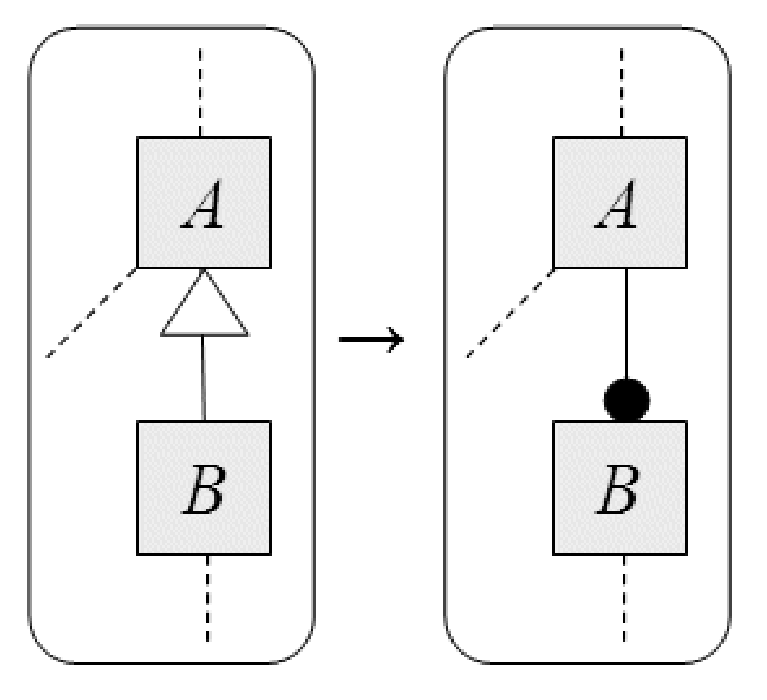
\includegraphics{images/bad-smell1.eps}}
\end{center}
\end{figure}

% template matching
Refactoring designers can apply general FM refactorings based on template matching. 
% templates
Each {\em general refactoring} consists of two {\em templates} (patterns) of FMs, on the left-hand (LHS) and right-hand (RHS) sides.
% quando podemos aplicar o refatoramento
A refactoring can be applied whenever the FM matches the template. A matching is an assignment of all meta-features occurring in the LHS template to concrete values.
% o que n�o e mostrado e igual nos dois modelos
Any element omitted by the templates remains unchanged, thus refactoring templates only show differences between FMs. 
% linhas pontilhadas
Moreover, a dashed line on top of a feature indicates that this feature may have a parent feature. A dashed line below a feature indicates that this feature may have additional subfeatures.

% o outro refactoring
A similar refactoring that converts an \emph{or} relation to a mandatory relation can be proposed. 
% corretude
Both refactorings and the following one can be shown correct using a encoding of FMs~\cite{Gheyi:2006aa} in Alloy~\cite{Jakson:2006aa} or using a Prototype Verification System (PVS)~\cite{Owre:2009aa} theory~\cite{Gheyi:2006aa-2}.

\subsection{Constraint imposing the selection of an alternative}

% 1. intuicao
Sometimes a constraint in the model may impose that a child of an alternative relation must always be selected. This bad smell occurs when a global constraint obligates the selection of an \emph{Alternative Feature} or \emph{Or Feature}.
% 2. porque � um problema?
\Fix{Leopoldo: sera que isto eh um problema quando nao eh uma feature
mandatoria que esta impondo a selecao de uma feature alternativa/or?} Since a child must always be selected, the other children of this relationship can never be selected. Detecting this kind of bad smell might reveal constraints that are inconsistent with the feature model relationships.

% 3. explicar em um exemplo toy
For instance, suppose that we add the constraint $B \Rightarrow D'$ in the feature model of Figure~\ref{fig:fm01}. Since B is a mandatory feature of A, it must be selected. From this fact and the previous constraint added, feature D' must be selected.  Therefore, only D' will be a valid option to the alternative feature D. The feature D'' can never be selected.
% conclusao
This may reveal a symptom of a bad design.
% 4. exemplo real

% 5. refatoramento
Refactoring~\ref{ref:ref2} removes this bad smell by excluding the constraint.

\begin{figure}[ht]
\begin{refine}{\ensuremath{\langle}change alternative constraint\ensuremath{\rangle}}
\label{ref:ref2}
\end{refine}
\begin{center}
\leavevmode
\scalebox{0.4}{
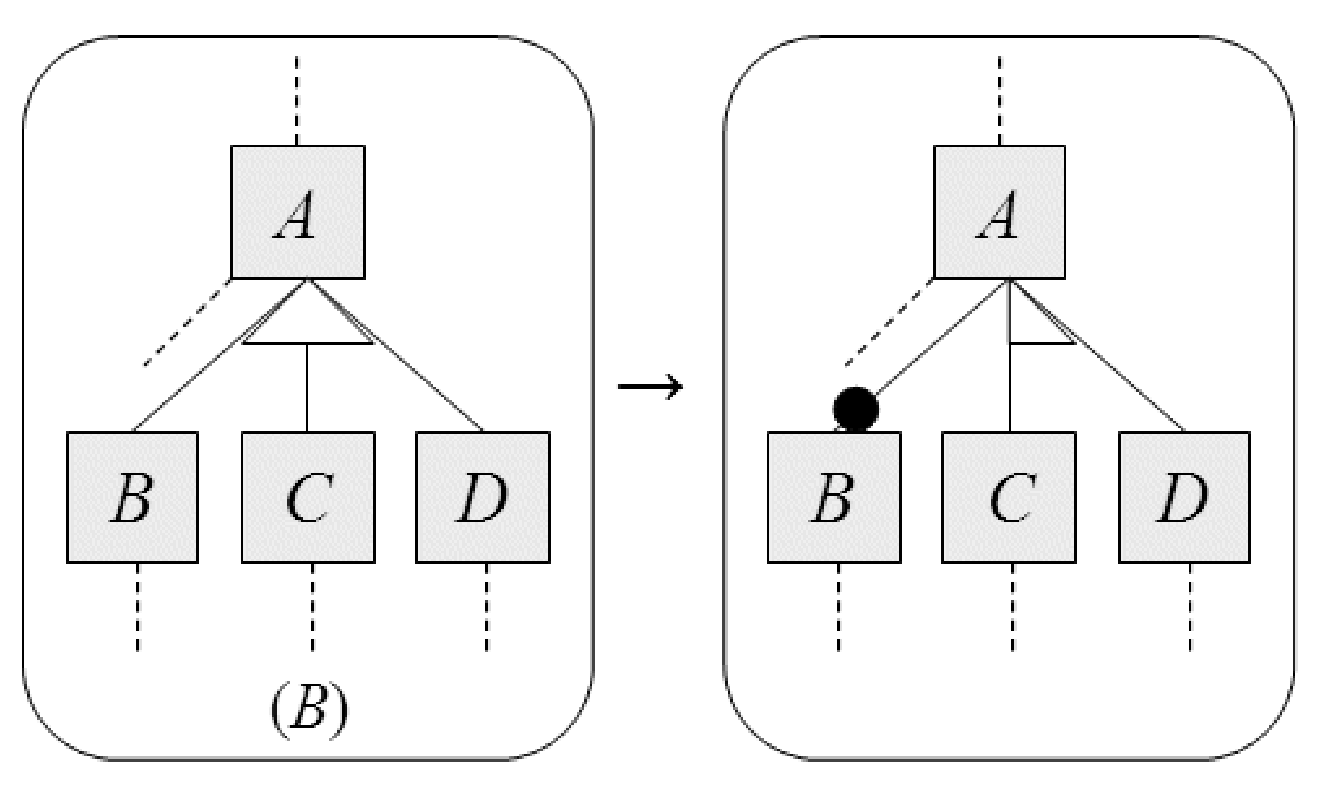
\includegraphics{images/bad-smell2.eps}}
\end{center}
\end{figure}

% refatoramento similar
A similar refactoring can be proposed for an \emph{Or} relationship.
% lei util
In this bad smell and in the following ones, which involve constraints (formulae), we may use Refactoring~\ref{ref:add-formula} in order to prepare the FM to match, for instance, Refactoring~\ref{ref:ref2} template. 
% explicando variavel
The \emph{fs} variable denotes a set of features.
% voltando ao exemplo
In the Figure~\ref{fig:fm01} feature model example, Refactoring~\ref{ref:add-formula} is used to deduce the constraint \emph{D'}. After that, we can apply Refactoring~\ref{ref:ref2}.

\begin{figure}[ht]
\begin{refine}{\ensuremath{\langle}add deducible formula\ensuremath{\rangle}}
\label{ref:add-formula}
\end{refine}
\begin{center}
\leavevmode
\scalebox{0.4}{
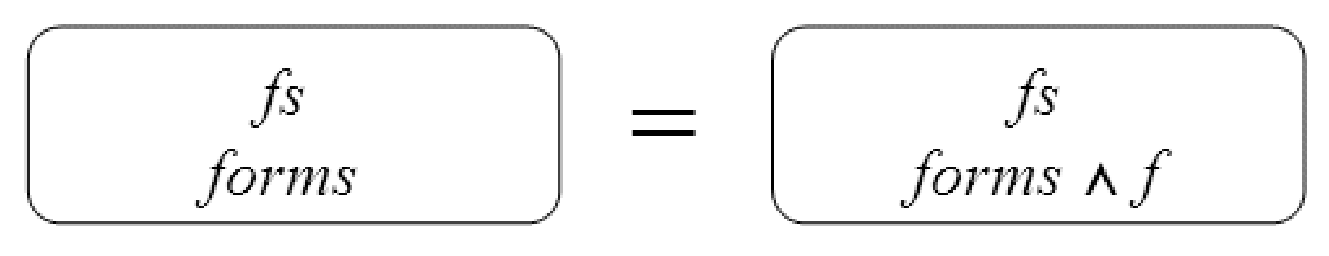
\includegraphics{images/add-formula.eps}}
\end{center}
\noindent ($\leftrightarrow$) \emph{f} can be deduced from \emph{forms} and \emph{fs}. \\
\end{figure}

\subsection{Constraint changing the semantics of a relationship}

% 1. intuicao
Sometimes a feature model may have a constraint making the semantics of a relationship more restrictive. 
% 2. porque � um problema?
This may waste time of domain analysts when understanding the model. It is better to change the relationship. It is easier to understand a model if we include most constraints in the graphical notation.
% 3. explicar em um exemplo toy
One example of this bad smell is present in the feature model of Figure~\ref{fig:fm01}.
As we explained in Section~\ref{sec:intro}, in the presence of the global constraint $B \Rightarrow D$, the optional relationship between the features A and D is changed to mandatory. Detecting this kind of bad smell reveals either an improper constraint or an inadequate feature model relationship.
% 4. exemplo real

% 5. refatoramento
This bad smell can be removed by applying Refactoring~\ref{ref:ref3}, which changes from the optional relationship to the mandatory relationship.

\begin{figure}[ht]
\begin{refine}{\ensuremath{\langle}replace optional to mandatory\ensuremath{\rangle}}
\label{ref:ref3}
\end{refine}
\begin{center}
\leavevmode
\scalebox{0.4}{
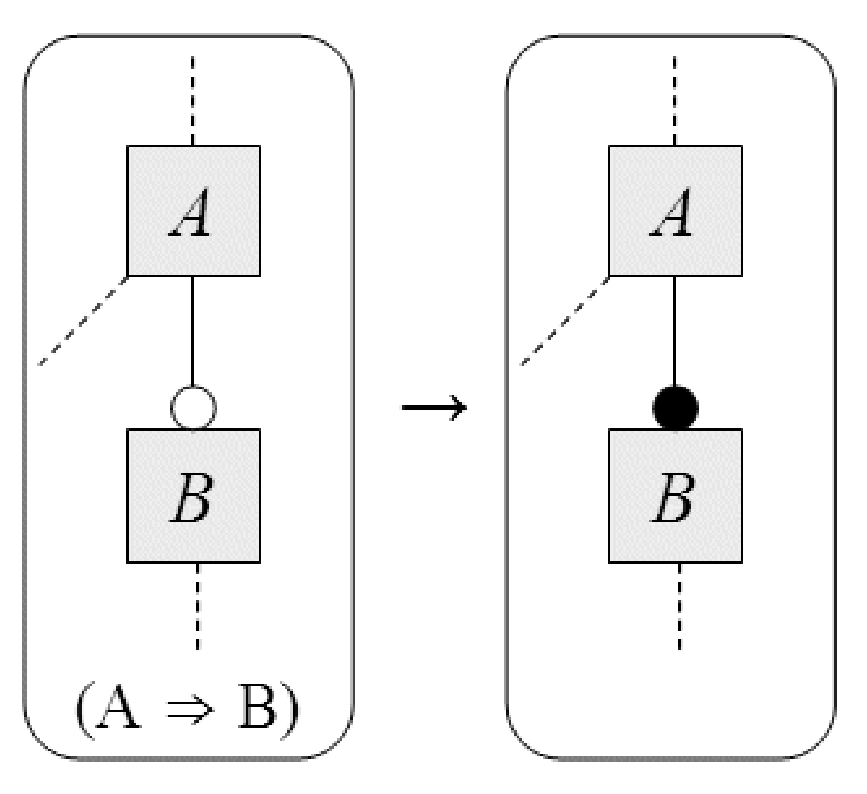
\includegraphics{images/bad-smell3.eps}}
\end{center}
\end{figure}

The same bad smell can appear between other relationships. For example, sometimes we can convert an \emph{Or} relationship to an \emph{Alternative} relationship. A number of refactorings can be useful for removing them~\cite{Gheyi:2009aa}.

\subsection{Redundant constraints}

% 1. intuicao
It is useful to add redundant constraints in order to make the model easier to understand. A redundant constraint does not narrow the number of instances (configurations) of a feature model --- so, it does not define any additional restriction to the feature model. The number of valid configurations is the same.
% 2. porque � um problema?
However, sometimes when we add a number of redundant constraints, it may be difficult for domain analysts to understand the entire model. They may waste time reading some constraints that does not add value to the model. So, in these situations, it may be better to remove them.

% 3. explicar em um exemplo toy
For example, suppose that one defines a constraint $C \Rightarrow B$ in the feature model of Figure~\ref{fig:fm01}, instead of writing a proper constraint. Note that such a constraint is redundant, since feature B must be present in any valid configuration of this feature model. 
% conclusao
Therefore, detecting this kind of bad smell might reveal a constraint that was not well specified. 
% 4. exemplo real
% 5. refatoramento
This bad smell can be removed by applying Refactoring~\ref{ref:add-formula} from right to left.

\subsection{Dead features}

% 1. intuicao
This bad smell occurs when a feature, due to a global constraint, could never be selected in the valid instances of a feature model~\cite{Trindad:2006aa}. It may happen because of the number of constraints in the model that may make the model difficult to understand, hence suitable for introducing errors.
% 2. porque � um problema?
This may be a symptom of a bad design. 

% 3. explicar em um exemplo toy
For instance, if the constraint $B \Rightarrow \neg C $ is added to the feature model of Figure~\ref{fig:fm01}, the feature C becomes a dead feature. It will never be present in any configuration of the feature model. 
% conclusao
If a feature is dead, it may be useless to the model and should be removed from it, or it may reveal a problem in the model (overconstrained) and we should remove some constraints.

% 4. exemplo real
% 5. refatoramento
Two refactorings can be used to remove this bad smell. Refactoring~\ref{ref:remove-formula} can be used to remove some constraints in the overconstrained model. 

\begin{figure}[ht]
\begin{refine}{\ensuremath{\langle}remove formula\ensuremath{\rangle}}
\label{ref:remove-formula}
\end{refine}
\begin{center}
\leavevmode
\scalebox{0.4}{
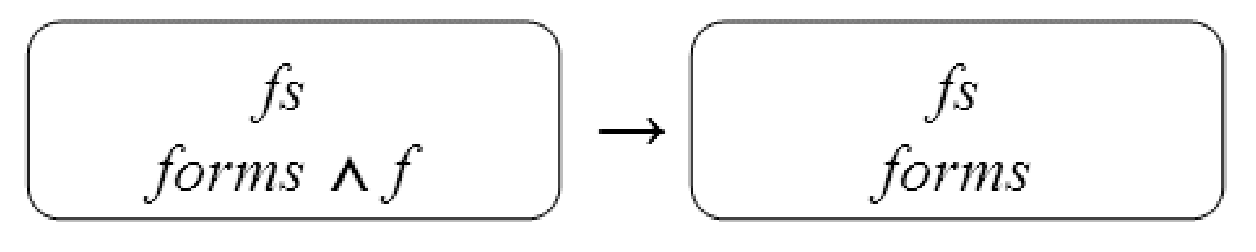
\includegraphics{images/remove-formula.eps}}
\end{center}
\end{figure}

In case the feature must be removed, we can apply Refactoring~\ref{ref:remove-feature}. We remove it from the model, and replace its occurrence in all constraints by \emph{false}.

\begin{figure}[ht]
\begin{refine}{\ensuremath{\langle}remove dead feature\ensuremath{\rangle}}
\label{ref:remove-feature}
\end{refine}
\begin{center}
\leavevmode
\scalebox{0.4}{
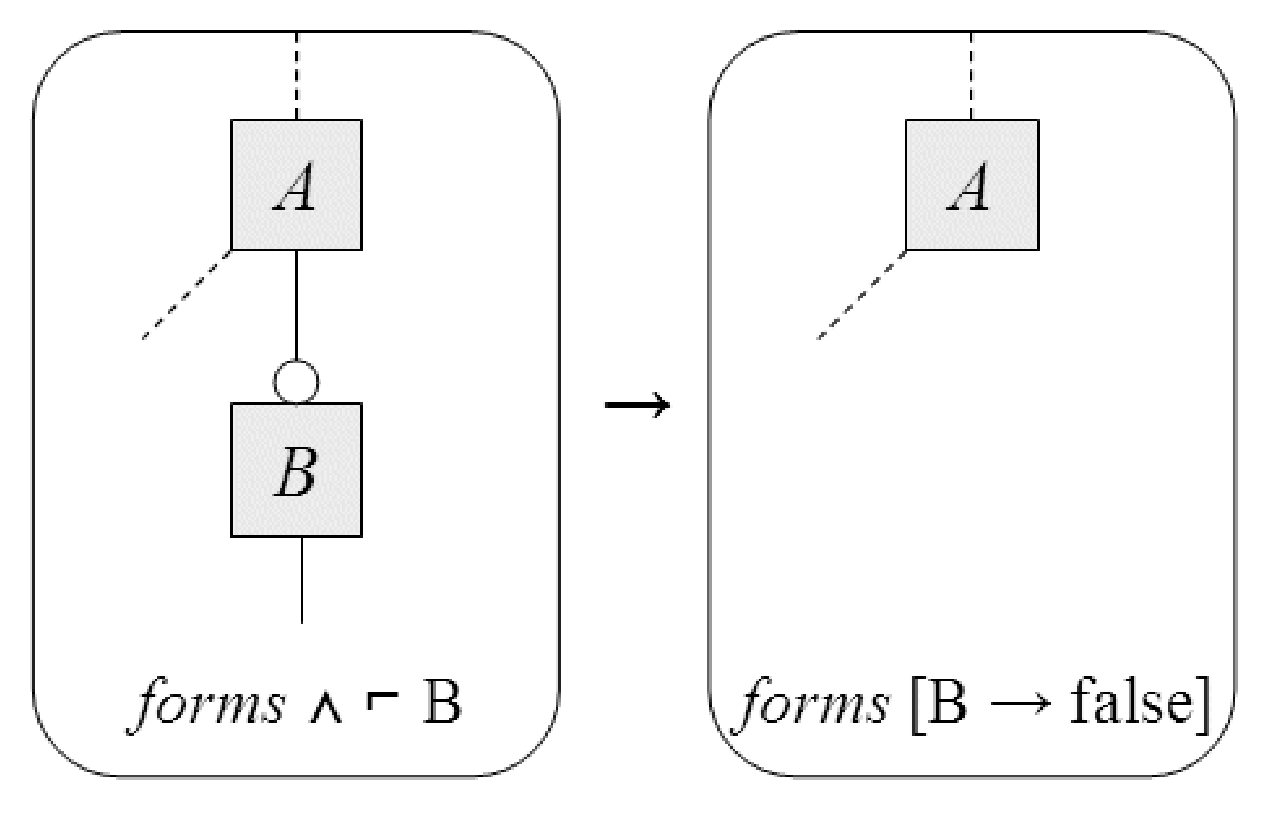
\includegraphics{images/remove-feature.eps}}
\end{center}
\end{figure}

\subsection{Inconsistent Model}

% 1. intuicao
This bad smell occurs when a feature model does not have any valid
configuration due to contradicting constraints. It may happen when
overconstraining the model, making it difficult to understand, hence, suitable
for introducing errors.
% 2. porque � um problema?
In general, this may be a symptom of a bad design and an error. 

% 3. explicar em um exemplo toy
For instance, if the constraint $C \Rightarrow \neg D $ is added to the feature
model of Figure~\ref{fig:fm01}, the model becomes inconsistent. The feature D
must always be selected.
% conclusao
If a model does not have a valid configuration, it may reveal an error in the
model design. In general, it is useless to have an inconsistent model.

% 4. exemplo real
% 5. refatoramento
In order to remove the contradiction, we first use a tool, such as proposed by Benavides~\cite{Trinidad:2008aa-2}, which extracts the minimum set of constraints that make the model inconsistent. After debugging the model, the domain analyst should check which set of constraints must be removed. Then, we can apply Refactoring~\ref{ref:remove-formula} to remove them from the model.



\section{Tool Support}\label{sec:tool-support}

We have developed a Haskell library and a set of tools for checking errors and bad smells in feature models. Therefore, offering these asserts to the Haskell community is another contribution of this work--- since, to our knowledge, there is no corresponding set of libraries and tools developed in functional languages. In short, these libraries and tools make available:

\begin{itemize}
 \item data types for feature modeling in Haskell;
 \item functions for checking if a feature model is well typed;
 \item functions for detecting bad smells in feature models;
 \item functions for checking if a feature model is satisfiable;
 \item functions for checking if a selection of features is a valid instance of a feature model; and
 \item integration with existing tools, such as Feature Modeling Plugin and FeatureIde 
\end{itemize}   

We start this section by presenting a few design decisions regarding the development of the feature model library. Then, we present some analysis of benchmarking that were performed on three distinct feature models available at~\cite{Group:2009yg}: \emph{eShop feature model} (325 features), \emph{Model transformation} (113 features) and \emph{Web portal} (49 features). These feature models have been widely described in the literature. We have also checked the satisfiability functions on models with 1000 features. 

\subsection{Design decisions}

For checking satisfiability, we have implemented two solutions. The first one is a purely functional implementation, using the Funsat Haskell library. Besides informing if a feature model is satisfiable or not, using this approach we can also get a valid instance for the model. However, this library is not optimized for complex feature models. For this reason, we have also developed an interface with the Minisat SAT solver, an open source project developed in C.    

\subsection{Benchmark analysis}

We evaluated our tools in small and medium-sized feature models that are publicly available. Since these models have been widely used in the literature, we believe that they are representative to our analysis. Basically, here we present  that our tools correctly detect errors and bad smells in reasonable time. Some of the existing models that we took already present some kind of error. Most of them are related to duplicated features. Bad smells were introduced in the evaluated feature models. 

For each feature model we evaluated three operations: type checker (TC), satisfiability checker (SC), and bad smells detection (BSD). Additionally, in order to reduce bias, we performed 50 evaluations for each pair \emph{operation and feature model}. We conducted all measurements on the same Mac OS-X with 2.16 GHz and 2 GB of RAM. The time, measured in milliseconds, was collected using the \emph{BenchPress} library~\cite{Tibell:2009rm}. The mean time for each pair is present in Table~\ref{tab:analysis}.

\begin{table}[htdp]
\begin{center}
\begin{tabular}{|l|c|c|c|c|} \hline
Feature model 			& Features 			& TC 	& SC 	& BSD      		\\ \hline
Web portal       			& 49                             	& 4.8 	& 4.5 	& 125.78 		\\ \hline
Model transformation       & 113			    	& 4.5	& 20.70	& 1339.03		\\ \hline 
eShop				& 325				& 15.27  	& 125.76	& 25806.05 	\\ \hline
\end{tabular}
\end{center}
\caption{Benchmark results}
\label{tab:analysis}
\end{table}

We can observe that the time required for detecting bad smells increases significantly as the number of features increase. For instance, checking bad smells in the \emph{eShop} feature model took approximately 25 seconds. This number is almost 20 times greater than the time required for detecting bad smells in the \emph{Model transformation} feature model. However, we claim that even in this case, the response time is reasonable, since it might significantly reduce the effort for detecting bad design decisions manually. Additionally, the current implementations of the corresponding functions were developed without considering performance. For instance, the function for detecting dead features (Listing~\ref{lst:dead})is extremely time consuming, since, for each optional feature, it makes a call for the satisfiability function. Optimizing these functions is a future activity. 

\begin{lstlisting}[belowskip=12pt,frame=tb,caption={Function for checking dead features.},label=lst:dead]
checkDeadFeatures :: FeatureModel -> [Feature]
checkDeadFeatures fm = 
 let fm' = addImplies fm
 in
  [ f | f <- features fm
  , isOptional f
  , not (isSatisfiable fm' f)
  ]
\end{lstlisting} 







  



  
 



\section{Evaluation}

% Discuss the benefits of applying the DR language in different case studies
% - Health watcher
% - choose one of the cases: TaRGeT, Games, Mobile Media, FLIP, \ldots
% Evaluate the benefits based on metrics
% - Concern metrics or Lattix Metrics

In this section we evaluate our language for specifying design rules
in AO systems. Basically, we discuss advantages and disadvantages of
using our approach when compared to other ones like Crosscutting
Programming Interfaces (XPIs). In what follows, we describe the
details of our evaluation:

%\begin{itemize}
%    \item[$\square$] hhh
%    \item[$\square$] aaa
%\end{itemize}

\subsection{Auditing Concern}

The auditing concern must be triggered when inserting, removing,
updating, or searching for a complaint.

Two teams working in parallel without design rules: the first one
works on the base code (the ComplaintRepository) and the second one
works on the auditing concern. Such a concern is implemented as an
aspect.

\scriptsize
\begin{lstlisting}[frame=single, caption={Complaint Repository implementation.},label=lst:complaint-repository, language=Java]
public class ComplaintRepository implements IComplaintRepository {

    public int insert(Complaint c) throws RepositoryException,
            ObjectAlreadyInsertedException {

    }

    public void update(Complaint c) throws RepositoryException,
            ObjectNotFoundException {

    }

    public void remove(int id) throws RepositoryException,
            ObjectNotFoundException {

    }

    public Complaint search(int id) throws RepositoryException,
            ObjectNotFoundException {

    }

}
\end{lstlisting}
\normalsize

Aspect for implementing the auditing concern:

\scriptsize
\begin{lstlisting}[frame=single, caption={Auditing Aspect.},label=lst:auditing-aspect, language=Java]
public aspect AuditingAspect {

    pointcut auditWhen():
           execution(int ComplaintRepository.insert(Complaint)
        || execution(void ComplaintRepository.update(Complaint)
        || execution(void ComplaintRepository.remove(int)
        || execution(Complaint ComplaintRepository.search(int)

    after() returning(): auditWhen() {
        // audit code.
    }

}
\end{lstlisting}
\normalsize

In the meanwhile, suppose that the teams are working on their
respective concerns (the repository and the auditing concerns). Now,
suppose that the team of the repository changes the following:

\begin{itemize}
    \item the insert method returns void instead of int; and

    \item the remove and search methods should take as parameter the
    Complaint object instead of an id.
\end{itemize}

Such changes might break the aspects...

% =================================== at� aqui entraria na se��o 2...

% ===== se��o 4

Design Rule:

\scriptsize
\begin{lstlisting}[frame=single, caption={Auditing Design Rule.},label=lst:auditing-dr, language=Java]
dr AuditingDesignRule {

    class ComplaintRepository {

        public int insert(Complaint c) throws RepositoryException,
                ObjectAlreadyInsertedException {}

        public void update(Complaint c) throws RepositoryException,
                ObjectNotFoundException {}

        public void remove(int id) throws RepositoryException,
                ObjectNotFoundException {}

        public Complaint search(int id) throws RepositoryException,
                ObjectNotFoundException {}

    }

    aspect AuditingAspect {

        pointcut auditWhen():
            execution(int ComplaintRepository.insert(Complaint)
            || execution(void ComplaintRepository.update(Complaint)
            || execution(void ComplaintRepository.remove(int)
            || execution(Complaint ComplaintRepository.search(int)

        % precisa do args aqui...??? Acho que sim...

        after() returning(): auditWhen() {
            xcall(void Auditing.auditComplaint(Complaint));
        }

    }

}
\end{lstlisting}
\normalsize

XPI of this example:

\textbf{Observa��o para colocar no texto: a XPI garante que n�o h�
chamadas fora do aspecto. No entanto, ela n�o garante:}

\begin{itemize}
    \item Que ocorre realmente uma chamada para auditComplaint;
    \item O local exato dessa chamada (dentro de um aspecto, por exemplo).
\end{itemize}

\scriptsize
\begin{lstlisting}[frame=single, caption={Auditing XPI.},label=lst:auditing-xpi, language=Java]
public aspect AuditingXPI {

    pointcut auditWhen():
        execution(int ComplaintRepository.insert(Complaint)
        || execution(void ComplaintRepository.update(Complaint)
        || execution(void ComplaintRepository.remove(int)
        || execution(Complaint ComplaintRepository.search(int)

    pointcut callToAudit(): call(void Auditing.auditComplaint(Complaint));

    declare error: (callToAudit() && !within(AuditingXPI)):
        "Contract violation: the auditComplaint method can not
        be called outside the aspect AuditingXPI";

}
\end{lstlisting}
\normalsize

In order to guarantee the contract that classes, aspects and their
respective methods and advices must exist, we can informally
document it like a prose, as mentioned in~\cite{sss}. Obviously, in
this case the contract is not verified by using the AspectJ
compiler, for instance.

However, we can guarantee the aforementioned contract by using
Aspect-Aware interfaces~\cite{sss}. Figure TAL illustrates that when
a pointcut does not match any piece of code, the compiler emits a
warning to the developer. Such a warning might be used to alert the
developer that some method must exist, for example.

\textbf{Observa��o para colocar no texto:}

As marca��es de AJDT (did not match) pode nos ajudar a identificar
classes ou m�todos que n�o existem. Mas elas n�o ajudam a
identificar que determinados aspectos ou advices existem.

Com quantifica��o, a AJDT consegue fazer as marca��es. No entanto,
ao remover um join point que � capturado pelo aspecto, nenhum erro �
apresentado (ou seja, n�o h� garantias que um determinado join point
existe ou n�o).

\subsection{Transaction Concern}

All methods of the HealthWatcherFacade must have transaction
management. In this case, due to the crosscutting nature of this
concern throughout the methods, we can use aspects to modularize it,
as showed in Listing TAL.

\scriptsize
\begin{lstlisting}[frame=single, caption={Transaction Management Aspect.},label=lst:transaction-aspect, language=Java]
public aspect HWTransactionManagement {

    pointcut transactionalMethods(): execution(* HealthWatcherFacade.*(..));

    after() returning: transactionalMethods()  {
        // ta errado... n�o � a interface
        IPersistenceMechanism.commitTransaction();
    }

    after() throwing: transactionalMethods()  {
        IPersistenceMechanism.rollbackTransaction();
    }

    before(): transactionalMethods() {
        IPersistenceMechanism.beginTransaction();
    }

}
\end{lstlisting}
\normalsize

\subsection{Concurrency Concern}

Section TAL showed the concurrency concern implemented as an aspect.
All methods of the \emph{EmployeeRepository} were synchronized by
the \emph{SynchronizationAspect}. In what follows, we present design
rules and XPIs to avoid modularity problems.

\scriptsize
\begin{lstlisting}[frame=single, caption={Concurrency Design Rule.},label=lst:concurrency-dr, language=Java]
dr Concurrency {

    class EmployeeRepository {

    }

    aspect SynchronizationAspect {

        pointcut concurrency(): execution(* EmployeeRepository.*(..));

        Object around(): concurrency() {

        }

    }

}
\end{lstlisting}
\normalsize

\subsection{Product Line Games}

\section[draft]{Related work}

Modularity issues in aspect-oriented programming have been reported by
different authors~\cite{sullivan-sigsoft-2005, leavens-observers-2002,
steiman-sigplan-2006}. For instance, Clifton and Leavens argue that
existing \emph{aspect-oriented} programming languages do not contribute to
comprehensibility, since they require systems to be studied in their entirety.
In order to improve comprehensibility of AOP systems, they propose a simple set
of restrictions that minimizes this problem~\cite{leavens-observers-2002}.

Steiman\ldots, \ldots . Other authors foccus on the discussion on how to expose
more stable aspect-oriented interfaces and how to compute module interfaces in
AOP systems. Since these later works are more related to our proposal, in the
remaining of this section we discuss them in more details\ldots


\subsection{Open Modules}

Open Modules is an approach for dealing with modularity issues in 
AOP~\cite{aldrich-ecoop-05}. Besides exposing data structures and 
functions, Open Modules' interfaces can also expose pointcuts denoting 
internal semantic of events. Clients of these modules are able to advice 
only exported pointcuts. Moreover, by exporting a pointcut, the module's 
developer is compromised to maintain the semantics of that pointcuts, 
which, in fact, mitigates the \emph{unantecipated changes} problem.
However, differently of our proposed language, Open Modules does not offers
mechanims for describing which are the responsabilities of aspect developers. As
a consequence, module developers are still able to implement part of a concern
assigned for a different team and they can not assume the existence of any
behavior expected to be modularized as an aspect.
 
\subsection{Crosscut Programming Interfaces}

The Crosscut Programming Interfaces (XPIs) is one attempt for defining design
rules between aspects and advised
code~\cite{sullivan-sigsoft-2005,sullivan-ieee-sw-2006}. Such interfaces specify
which are the exposed join-points of a base code. Although just an abstract XPI
representation was provided in~\cite{sullivan-sigsoft-2005}, Griswold et. al
presented how to implement crosscutting interfaces as syntactic constructs of
AspectJ~\citet{sullivan-ieee-sw-2006}. Based on this approach, design rules are
documented using \emph{abstract pointcut descriptions} and constraints applied to
the base code. These constraints might be written as \emph{declare warning} (or
\emph{declare error}) constructs or just as comments in the source code (when a
constraint can not be expressed as a \emph{declare warning} or \emph{declare
error}). 

XPIs authors argue that the main advantages of their approach is that:
(a) it does not require any new construct in the AspectJ language; and (b) there
is no restriction to the pointcut visibility. In fact, this characteristic
encourage the use of XPIs in sites that are already using the AspectJ language.
However, most of the constraints required for defining the responsibilities of
both class developers and aspect developers can not be checked using the proposed
XPI language (a deeper comparison of our approach against XPIs is presented in
Section~\ref{sec:eval}). Consequently, it is not possible to guarantee, at least
automatically, if certain design rules are being obeyed. 

For instance, we can not
express, using AspectJ constructs, that a call to a method \emph{must} occurs
within the control flow of another method. Actually, we can define such a
pointcut, but if it does not exist,  no error is reported by the AspectJ
compiler. Actually, pointcut constructs in AspectJ were proposed for specifying
points of execution that should be augmented by advices. They were not proposed
for specifying restrictions applied for base code developing.

\subsection{Aspectaware Interfaces}
% Aiming at specifying restrictions in base code using AspectJ like languages,
% developers are able to check if a {\bf non desirable} pointcut occurs in the
% source code (by means of \emph{declare error} or {declare warning} constructs).
% However, there is no construct which can be used for specifying that a specific
% pointcut {\bf must} occur in the source code. However, in order to improve
% modularity between crosscutting and base decisions, it is necessary to define
% what is expected from both teams (not only what aspect developers require, as
% supported by XPIs).


\section{Concluding Remarks}

% a summary of the main concluding remarks 
% of the paper.




% An example of a floating figure using the graphicx package.
% Note that \label must occur AFTER (or within) \caption.
% For figures, \caption should occur after the \includegraphics.
% Note that IEEEtran v1.7 and later has special internal code that
% is designed to preserve the operation of \label within \caption
% even when the captionsoff option is in effect. However, because
% of issues like this, it may be the safest practice to put all your
% \label just after \caption rather than within \caption{}.
%
% Reminder: the "draftcls" or "draftclsnofoot", not "draft", class
% option should be used if it is desired that the figures are to be
% displayed while in draft mode.
%
%\begin{figure}[!t]
%\centering
%\includegraphics[width=2.5in]{myfigure}
% where an .eps filename suffix will be assumed under latex, 
% and a .pdf suffix will be assumed for pdflatex; or what has been declared
% via \DeclareGraphicsExtensions.
%\caption{Simulation Results}
%\label{fig_sim}
%\end{figure}

% Note that IEEE typically puts floats only at the top, even when this
% results in a large percentage of a column being occupied by floats.


% An example of a double column floating figure using two subfigures.
% (The subfig.sty package must be loaded for this to work.)
% The subfigure \label commands are set within each subfloat command, the
% \label for the overall figure must come after \caption.
% \hfil must be used as a separator to get equal spacing.
% The subfigure.sty package works much the same way, except \subfigure is
% used instead of \subfloat.
%
%\begin{figure*}[!t]
%\centerline{\subfloat[Case I]\includegraphics[width=2.5in]{subfigcase1}%
%\label{fig_first_case}}
%\hfil
%\subfloat[Case II]{\includegraphics[width=2.5in]{subfigcase2}%
%\label{fig_second_case}}}
%\caption{Simulation results}
%\label{fig_sim}
%\end{figure*}
%
% Note that often IEEE papers with subfigures do not employ subfigure
% captions (using the optional argument to \subfloat), but instead will
% reference/describe all of them (a), (b), etc., within the main caption.


% An example of a floating table. Note that, for IEEE style tables, the 
% \caption command should come BEFORE the table. Table text will default to
% \footnotesize as IEEE normally uses this smaller font for tables.
% The \label must come after \caption as always.
%
%\begin{table}[!t]
%% increase table row spacing, adjust to taste
%\renewcommand{\arraystretch}{1.3}
% if using array.sty, it might be a good idea to tweak the value of
% \extrarowheight as needed to properly center the text within the cells
%\caption{An Example of a Table}
%\label{table_example}
%\centering
%% Some packages, such as MDW tools, offer better commands for making tables
%% than the plain LaTeX2e tabular which is used here.
%\begin{tabular}{|c||c|}
%\hline
%One & Two\\
%\hline
%Three & Four\\
%\hline
%\end{tabular}
%\end{table}


% Note that IEEE does not put floats in the very first column - or typically
% anywhere on the first page for that matter. Also, in-text middle ("here")
% positioning is not used. Most IEEE journals/conferences use top floats
% exclusively. Note that, LaTeX2e, unlike IEEE journals/conferences, places
% footnotes above bottom floats. This can be corrected via the \fnbelowfloat
% command of the stfloats package.

% use section* for acknowledgement
\section*{Acknowledgment}

The authors would like to thank...more thanks here


% trigger a \newpage just before the given reference
% number - used to balance the columns on the last page
% adjust value as needed - may need to be readjusted if
% the document is modified later
%\IEEEtriggeratref{8}
% The "triggered" command can be changed if desired:
%\IEEEtriggercmd{\enlargethispage{-5in}}

% references section

\bibliographystyle{abbrv}
\bibliography{splc2009}






% that's all folks
\end{document}


